\documentclass[a4paper]{article}

\usepackage{mathrsfs}
% ============================================
%         General Packages
% ============================================
\usepackage{balance}

\usepackage{kotex}      % for Korean
\usepackage{lipsum}     % for dummy text
\usepackage{array}

\usepackage{cite}   % for citation

\usepackage{amsmath,amsfonts}
\usepackage{amssymb}
\usepackage{soul}
\usepackage{mathrsfs}

\usepackage{hyperref}

    \hypersetup{
        pdftoolbar=false,        	% show Acrobat’s toolbar?
        pdfmenubar=false,        	% show Acrobat’s menu?
        pdffitwindow=false,     	% window fit to page when opened
        pdfstartview={FitH},    	% fits the width of the page to the window
        pdftitle={},    	% title
        pdfauthor={},     	% author
        %     pdfsubject={},   	% subject of the document
        %     pdfcreator={},   	% creator of the document
        %     pdfproducer={}, 	% producer of the document
        %     pdfkeywords={keyword1, key2, key3}, % list of keywords
        %     pdfnewwindow=true,      	% links in new PDF window
        colorlinks=true,       	% false: boxed links; true: colored links
        linkcolor=blue,          	% color of internal links (change box color with linkbordercolor)
        citecolor=blue,       	% color of links to bibliography
        filecolor=blue,      	% color of file links
        urlcolor=blue		% color of external links
    }

\usepackage{algorithm}
\usepackage{algorithmic}

\usepackage{epsfig}
\usepackage[dvipsnames]{xcolor}

% MY PACKAGES ===================================

\usepackage{svg}
\usepackage{subfig}

\usepackage{textcomp}
\usepackage{stfloats}
\usepackage{url}
\usepackage{verbatim}
\usepackage{graphicx}
\usepackage{multirow}
\usepackage{multicol}

\let\proof\relax
\let\endproof\relax
\usepackage{amsthm}
\usepackage{lipsum}
\usepackage{tikz}

% 
\usepackage{titlepic}
\usepackage{pdfpages}
\usepackage{etoolbox} % 조건문을 쓰기 위한 패키지


\titlepic{%
  
\includegraphics[height = 8mm]{figures/logo_KAIST_simple.png}
  \hspace{5mm}
  
\includegraphics[height = 8mm]{figures/MIC_Logo.png}
  }

% ========================================
%         TITLE and AUTHORS
% ========================================
\title{
  Constrained PINN
}

\author{
    Seunghun Jang
    \thanks{\href{https://kaist-mic-lab.github.io/members/shJang/}{Seunghun Jang} is Ph.D. student at KAIST, {\tt\small shjang7071@kaist.ac.kr}}%
}

\date{
    % 20\textsuperscript{th} March 2025
    Complied on \today
}

\begin{document}

\maketitle

% ========================================
%         Contents
% ========================================

\begin{figure}[h]
  \centering
  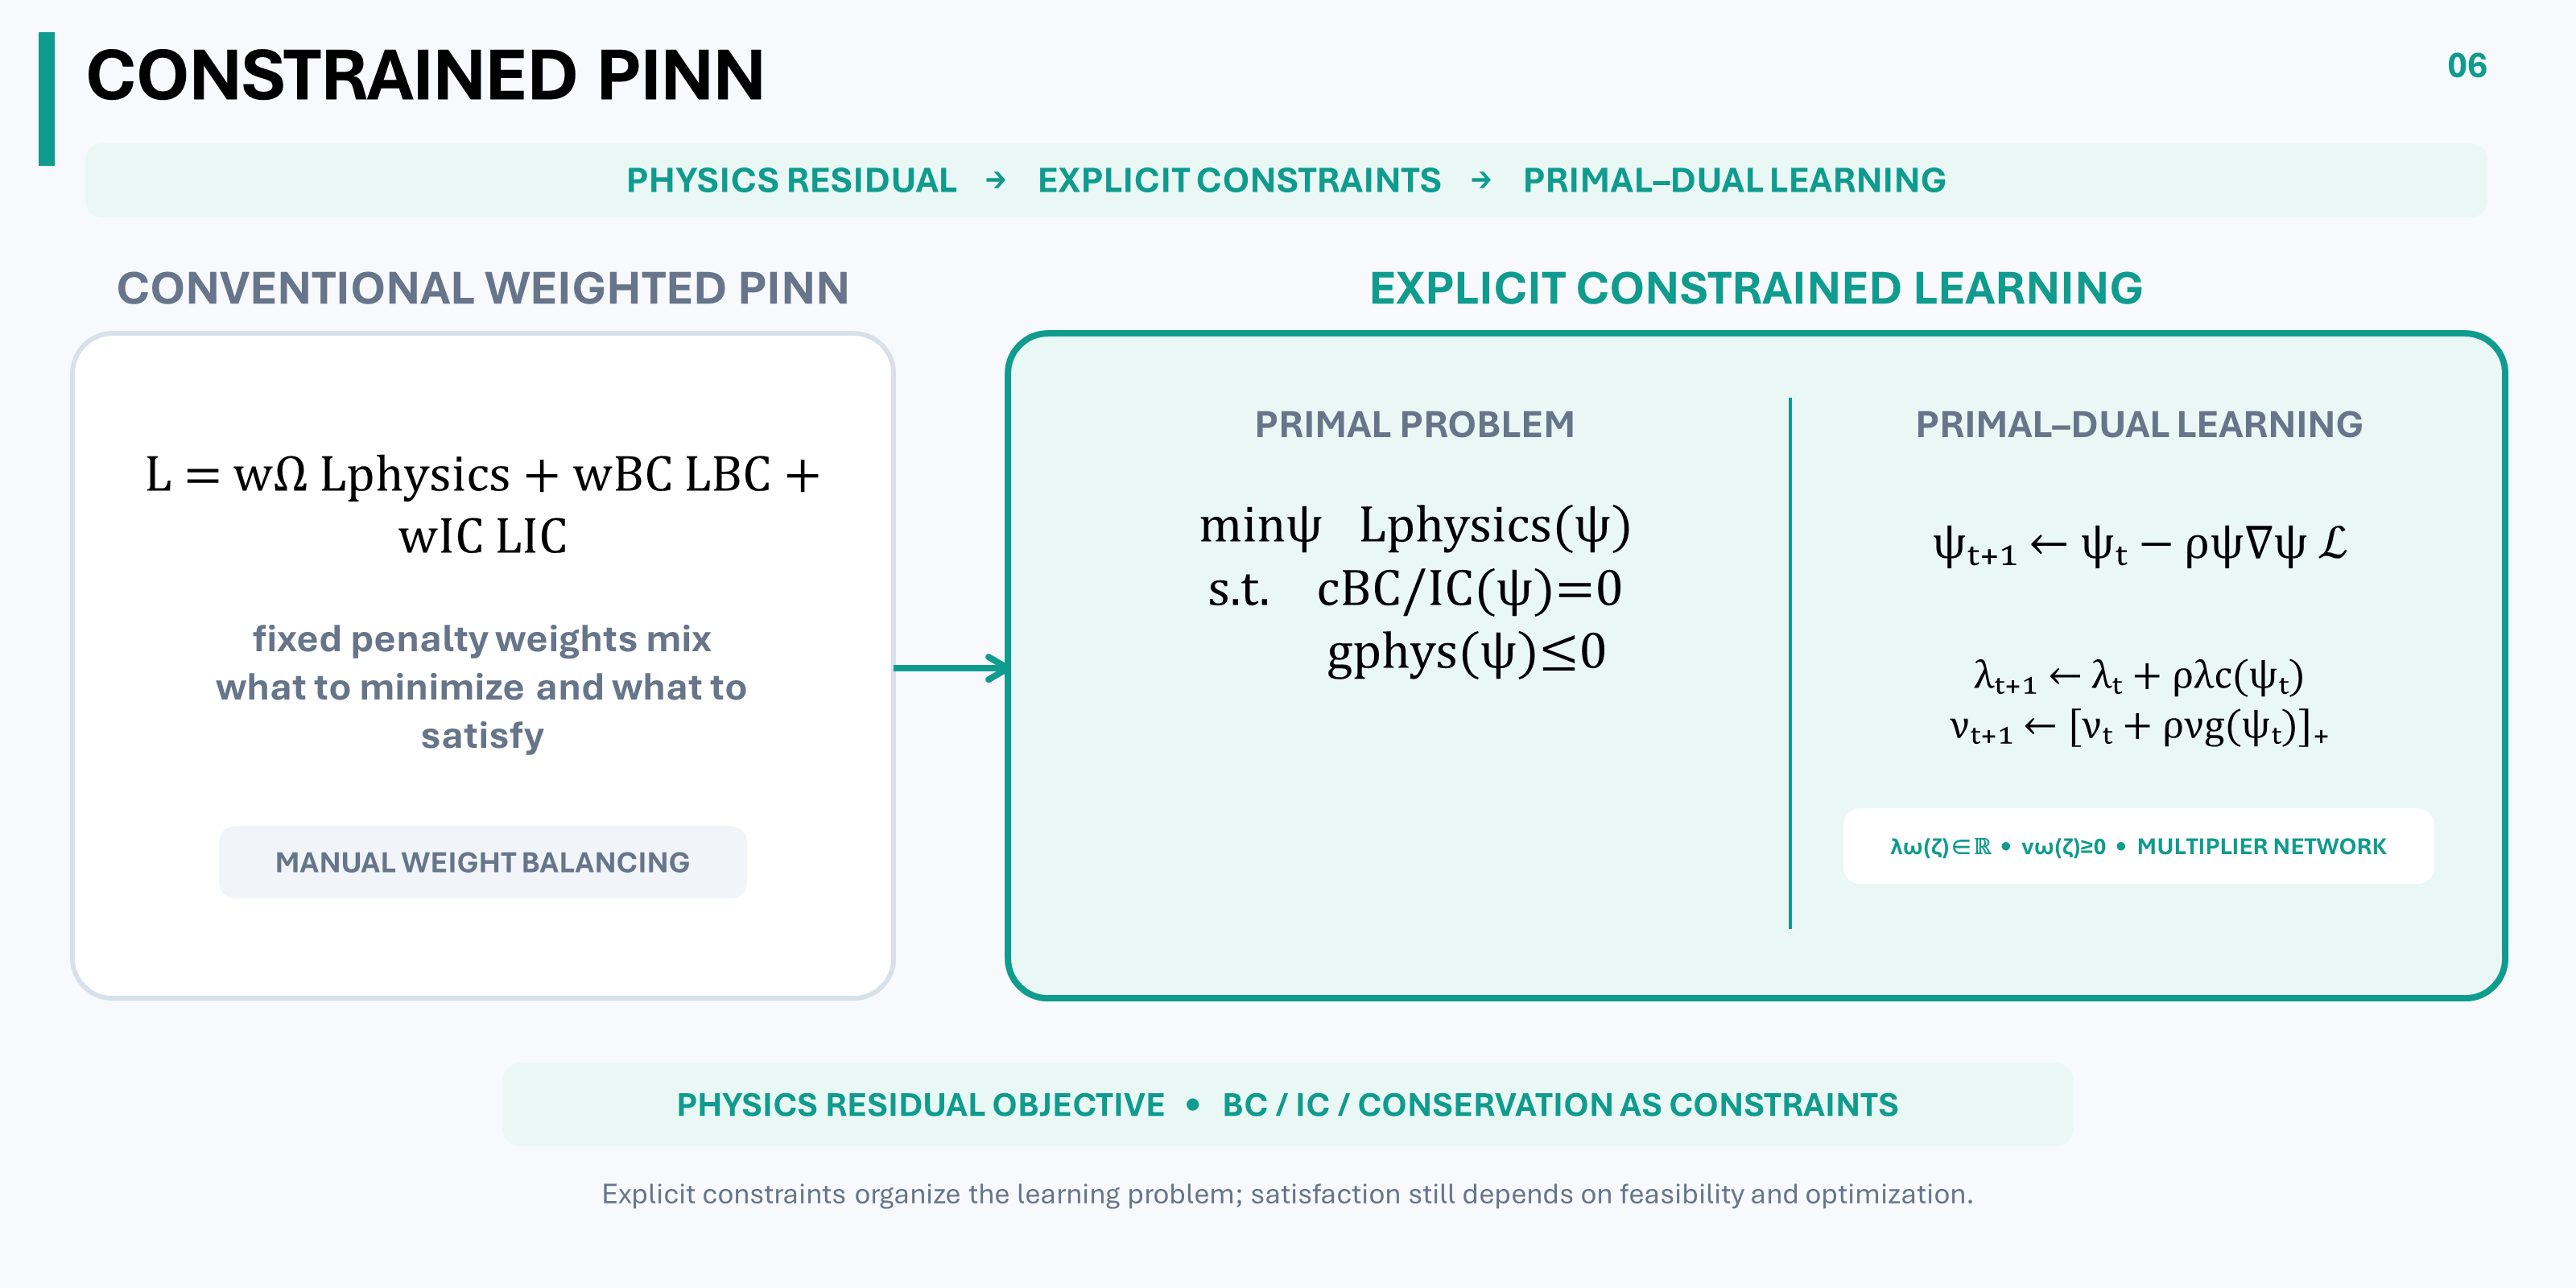
\includegraphics[width=\textwidth]{figures/06_constrained_pinn.png}
  \caption{Physics and data define an explicit constrained learning problem whose primal and dual variables produce a physics-consistent field or model.}
\label{fig:}
\end{figure}
The formulation distinguishes sampled residual minimization from
continuous-domain constraint satisfaction. Writing an explicit constraint
does not by itself establish feasibility or convergence.

\section{Problem definition}

This Theme concerns the model and state-information side of
\href{https://kaist-mic-lab.github.io/research/research_themes/RT_research_themes/}{Online Learning-Based Optimal Control},
but PINNs also apply well beyond control. It therefore begins from the general
problem of learning a physical field or model rather than from a Bellman
decision problem.

Within the MIC Lab program, Constrained PINN is primarily a supporting
physics-learning capability: it can prepare or update a control-usable model
or state representation for an online estimator, predictor, critic target, or
controller.

Let $q$ denote the physical field or model and let
$\widehat q_\psi(\zeta)$ be its primal neural approximation, parameterized by
$\psi$. The coordinate $\zeta$ may contain space, time, geometry, material
parameters, and operating conditions. For a governing operator $\mathcal N$,
define the interior physics residual

\begin{equation}
r_\Omega(\zeta;\psi)
=
\mathcal N
\!\left(
\widehat q_\psi
\right)(\zeta)
-
b(\zeta),
\end{equation}

where $b(\zeta)$ is the declared source or forcing term. Let
$\mathcal C_\Omega$ be the interior collocation set; the corresponding loss is

\begin{equation}
\mathcal L_{\mathrm{physics}}(\psi)
=
\frac{1}{|\mathcal C_\Omega|}
\sum_{\zeta\in\mathcal C_\Omega}
\left\|
r_\Omega(\zeta;\psi)
\right\|^2.
\end{equation}

For a forward problem, set
$\mathcal L_{\mathrm{obj}}=\mathcal L_{\mathrm{physics}}$. For an inverse
problem or sparse-data reconstruction, an observation term may be included:

\begin{equation}
\mathcal L_{\mathrm{obj}}(\psi)
=
\mathcal L_{\mathrm{physics}}(\psi)
+
w_{\mathrm{obs}}\mathcal L_{\mathrm{obs}}(\psi),
\qquad
w_{\mathrm{obs}}\ge0.
\end{equation}

The observation term remains part of the objective rather than one of the
declared physical constraints. Here $\mathcal L_{\mathrm{obs}}$ denotes the
observation-data misfit.

Boundary, initial, conservation, interface, and admissibility conditions are
represented as equality and inequality residuals:

\begin{equation}
c_j(\zeta;\psi)=0
\quad \forall\zeta\in\mathcal C_j^{=},
\qquad
d_m(\zeta;\psi)\le0
\quad \forall\zeta\in\mathcal C_m^{\le}.
\end{equation}

Here $j=1,\ldots,J$ and $m=1,\ldots,M$. Scalar residuals are shown for
clarity; components of vector-valued residuals are stacked in the same way.
The sets $\mathcal C_j^{=}$ and $\mathcal C_m^{\le}$ specify where sampled
equality and inequality constraints are enforced.

For example,

\begin{equation}
\begin{aligned}
c_{\mathrm{BC}}(\zeta;\psi)
&=
\mathcal B\!\left(\widehat q_\psi\right)(\zeta)
-
b_{\partial\Omega}(\zeta),\\
c_{\mathrm{IC}}(s;\psi)
&=
\widehat q_\psi(s,0)-q_0(s).
\end{aligned}
\end{equation}

$\mathcal B$ is the boundary operator, $b_{\partial\Omega}$ is the prescribed
boundary data, and $q_0$ is the initial field over the spatial coordinate $s$.

The defining optimization problem places the physics residual and any
observation loss in the objective, and the remaining requirements after an
explicit $\mathrm{s.t.}$ line:

\begin{equation}
\begin{aligned}
\min_{\psi}\quad
&\mathcal L_{\mathrm{obj}}(\psi)\\
\mathrm{s.t.}\quad
&c_j(\zeta;\psi)=0
\quad \forall\zeta\in\mathcal C_j^{=},\\
&d_m(\zeta;\psi)\le0
\quad \forall\zeta\in\mathcal C_m^{\le}.
\end{aligned}
\end{equation}

This equation defines the target learning problem, not a training algorithm.
For the sampled problem, each pair $(j,\zeta)$ in an equality collocation set
has an unrestricted multiplier, and each pair $(m,\zeta)$ in an inequality
collocation set has a nonnegative multiplier. Stacking them gives the dual
vectors $\lambda$ and $\nu$, respectively. Section 5 first gives direct vector
updates and then an optional shared \textbf{multiplier-network} parameterization
that generates these entries from $\zeta$.

\section{Why this problem matters}

PINNs can learn complex fields or models by combining sparse observations
with governing physics. A conventional PINN usually places PDE residuals,
boundary conditions, initial conditions, data, and conservation terms in one
weighted sum. Large differences in scale and conditioning can cause training
to reduce one term while leaving another physically important condition
poorly satisfied.

An explicit constrained formulation separates what should be minimized from
what should be satisfied. With appropriate residual scaling, convergence, and
constraint qualifications, the associated Lagrange multipliers can provide
local sensitivity information, and nonzero inequality multipliers can help
identify active constraints. Raw magnitudes are not directly comparable
across differently scaled residuals. This can make the learning problem more
transparent and reduce manual penalty-weight tuning, but it does not
automatically produce an exact physical solution or a convergent algorithm.

\section{Key challenges}

\begin{itemize}
  \item \textbf{Feasibility and representation:} the network class, collocation set, and
  coupled physical conditions may not admit a feasible solution.
  \item \textbf{Nonconvex primal--dual learning:} simultaneous primal-network and dual
  updates can oscillate, diverge, or become poorly scaled.
  \item \textbf{Sampled versus continuous satisfaction:} small residuals at collocation
  points do not prove physical consistency throughout the domain or under new
  conditions.
  \item \textbf{Multiplier representation and computation:}\\
  independently optimized
  pointwise multipliers scale with the collocation set; a shared multiplier
  network adds approximation choices, regularization, gradient-computation
  cost, and another coupled learning problem.
\end{itemize}

\section{Baselines --- weighted penalties and hard parameterization}

The standard soft-penalty PINN minimizes

\begin{equation}
\begin{aligned}
\mathcal L_{\mathrm{pen}}(\psi)
={}&
w_\Omega\mathcal L_{\mathrm{physics}}(\psi)
+w_{\mathrm{BC}}\mathcal L_{\mathrm{BC}}(\psi)\\
&+w_{\mathrm{IC}}\mathcal L_{\mathrm{IC}}(\psi)
+\sum_r w_r\mathcal L_r(\psi),\\
&w_\Omega,w_{\mathrm{BC}},w_{\mathrm{IC}},w_r\ge0.
\end{aligned}
\end{equation}

$\mathcal L_{\mathrm{BC}}$ and $\mathcal L_{\mathrm{IC}}$ are the sampled
boundary- and initial-residual losses, while $r$ indexes any additional
residual penalties.

Fixed weights are simple, and adaptive loss balancing can reduce some scale
mismatch. Nevertheless, a finite penalty permits constraint violation,
whereas a very large penalty can make optimization ill-conditioned.

For a selected simple equality condition, a separate hard baseline is

\begin{equation}
\widehat q_\psi(\zeta)
=
q_{\mathrm{known}}(\zeta)
+
A(\zeta)h_\psi(\zeta)
\end{equation}

This parameterization is chosen \textbf{before training}, rather than applied as a
correction afterward. Here $q_{\mathrm{known}}$ satisfies the prescribed
condition, $h_\psi$ is an unconstrained neural correction, and $A(\zeta)$ is
zero wherever that value condition must hold. For example, the initial
condition $q(s,0)=q_0(s)$ can be encoded as

\begin{equation}
\widehat q_\psi(s,\tau)
=
q_0(s)+\tau h_\psi(s,\tau).
\end{equation}

At physical time $\tau=0$, the neural correction vanishes for every $\psi$,
so the initial condition remains exactly satisfied throughout training. For a
derivative or operator constraint, $A=0$ alone is insufficient: the
parameterization must make the relevant operator applied to the correction
vanish. Hard encoding is therefore useful for selected simple equalities but
can be difficult to construct for complex geometries, coupled interfaces,
inequalities, or changing conditions.

\section[Research direction --- explicit constraints and primal--dual learning]
{Research direction ---\\ explicit constraints and primal--dual learning}

At the sampled level, stack equality and inequality residuals over their
collocation sets as $c(\psi)$ and $d(\psi)$. The Lagrangian is

\begin{equation}
\mathscr L(\psi,\lambda,\nu)
=
\mathcal L_{\mathrm{obj}}(\psi)
+
\lambda^\top c(\psi)
+
\nu^\top d(\psi),
\qquad
\nu\ge0.
\end{equation}

At primal--dual training iteration $t$, distinct from the physical coordinate
$\tau$ used above, conceptual updates are

\begin{equation}
\begin{aligned}
\psi_{t+1}
&=
\psi_t
-
\rho_{\psi,t}
\nabla_\psi
\mathscr L(\psi_t,\lambda_t,\nu_t),\\
\lambda_{t+1}
&=
\lambda_t
+
\rho_{\lambda,t}c(\psi_t),\\
\nu_{t+1}
&=
\left[
\nu_t
+
\rho_{\nu,t}d(\psi_t)
\right]_+ .
\end{aligned}
\end{equation}

Here $\rho_{\psi,t},\rho_{\lambda,t},\rho_{\nu,t}>0$, and $[\cdot]_+$ denotes
componentwise projection onto the nonnegative orthant. Equality multipliers
$\lambda$ are unrestricted, so their update is signed. The projected
inequality update increases a multiplier for positive violation and can
decrease it when the corresponding constraint is strictly satisfied. The
primal step updates the learned field or model.
Augmented-Lagrangian terms, residual normalization, alternating updates, and
dual regularization are possible stabilization mechanisms rather than
guarantees.

The updates above optimize one multiplier entry per sampled residual. Shared
\textbf{multiplier networks} can instead generate domain-indexed entries:

\begin{equation}
\lambda_j(\zeta)
=
\Lambda_{\omega_\lambda,j}(\zeta),
\qquad
\nu_m(\zeta)
=
\operatorname{softplus}
\!\left(
R_{\omega_\nu,m}(\zeta)
\right)
\ge0.
\end{equation}

$\Lambda_{\omega_\lambda,j}$ is the equality-network output, and
$R_{\omega_\nu,m}$ is the raw inequality-network output, with
$\omega_\lambda$ and $\omega_\nu$ denoting their parameters. The equality
multiplier needs no sign transformation, while softplus enforces
$\nu_m\ge0$. At each collocation batch, these outputs supply $\lambda$ and
$\nu$ in the sampled Lagrangian; $\psi$ is updated by descent and the
multiplier-network parameters by dual ascent. This shares a parameterization
across points but restricts the dual class, so sampled feasibility still does
not establish continuous-domain feasibility.

Future evidence should compare a baseline PINN, fixed and adaptive penalties,
hard encoding where available, directly optimized multiplier vectors with
standard or augmented-Lagrangian updates, and a multiplier-network variant
under matched data and computation budgets.
Metrics should include reference-solution error, physics residual, mean and
maximum constraint violation, conservation defect, training stability,
multiplier behavior, computation, and generalization to new boundary
conditions, parameters, and geometries.

\section{Application domains}

\begin{itemize}
  \item \textbf{Structural, contact, and multiphysics systems}, where interface,
  conservation, positivity, or material conditions must be distinguished
  from the governing residual objective.
  \item \textbf{Sparse-observation inverse problems and state reconstruction}, where
  physical constraints supplement incomplete measurements.
  \item \textbf{Synchronous-machine flux-linkage learning and estimation}, where
  governing electrical dynamics and physically admissible inductance bounds
  guide online learning of a nonlinear magnetic model. A related MIC Lab study
  reports simulation validation on a 35-kW IPMSM drive
  (\href{https://ieeexplore.ieee.org/document/11221587/}{Jang, Ryu, and Choi, 2025}).
  \item \textbf{EV battery and thermal-management analysis},\\
  including temperature-field
  reconstruction under changing cooling conditions and sparse sensing.
\end{itemize}

\section{References}

\begin{itemize}
  \item S. Jang, M. Ryu, and K. Choi, ``Physics-Informed Online Learning of Flux
  Linkage Model for Synchronous Machines,'' \textit{IECON 2025 --- 51st Annual
  Conference of the IEEE Industrial Electronics Society}, pp. 1--6, 2025.
  \href{https://ieeexplore.ieee.org/document/11221587/}{IEEE Xplore}
  \quad \href{https://kaist-mic-lab.github.io/static/pub/2025-physics-informed-IECON.pdf}{Full text}
\end{itemize}

\end{document}
